\newpage
\appendix
\onecolumn
\section{More Experiments}
\subsection{Hyper-Parameters} 
\label{hyperparameter}
We adopt the hyperparameter settings from HLFormer \cite{HLFormer} and GMMFormerV2 \cite{GMMFormerV2}. The numbers of clips and frames are set to $M_c=32$ and $M_f=128$, respectively. The maximum query length $N_q$ is fixed to 64 for ActivityNet Captions and 30 for TVR and Charades-STA. All remaining settings, including $L_{\text{sim}}$ and $L_{\text{div}}$, follow \cite{HLFormer}. Detailed implementation can be provided in the submitted code \href{https://github.com/lijun2005/ICML26-Holmes}{ICML26-Holmes}.


\subsection{Parameter Analysis}
We performed a comprehensive hyperparameter analysis on the TVR dataset to investigate the effects of the temperature $\tau$ in \cref{ea:evi1}, the threshold $\beta$ in \cref{eq:threshold}, and the dustbin bucket ratio $z$ in \cref{eq:new-s}, as depicted in \cref{fig:parameter_analysis}. The results indicate that our model maintains relatively stable performance when $\tau$ is within [0.06, 0.2], $\beta$ within [0.2, 0.5], and $z$ within [0.2, 0.4], demonstrating that the proposed approach is largely insensitive to hyperparameter variations and exhibits strong robustness.

\begin{figure*}[h]
    \centering
    \vspace{-0.8em}
    \parbox[b]{0.25\textwidth}{
        \centering
            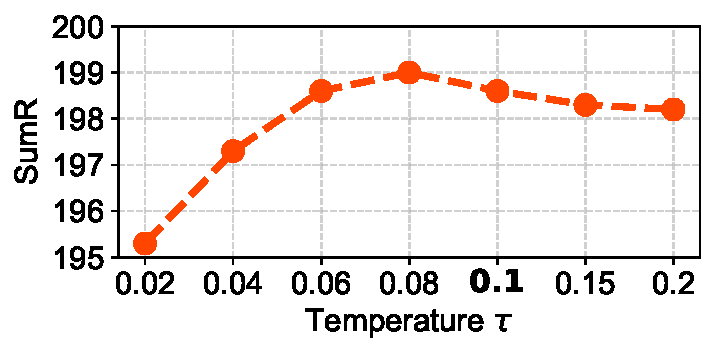
\includegraphics[width=\linewidth]{images/tvr_tau-.pdf}
    }
    \hspace{0.02\textwidth}
    \parbox[b]{0.25\textwidth}{
        \centering
            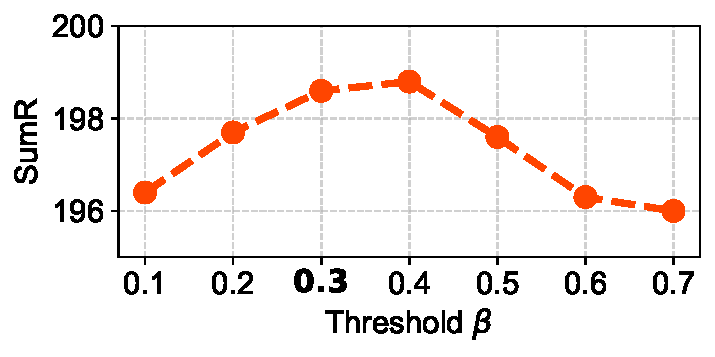
\includegraphics[width=\linewidth]{images/tvr_beta-.pdf}
    }
    \parbox[b]{0.25\textwidth}{
        \centering
            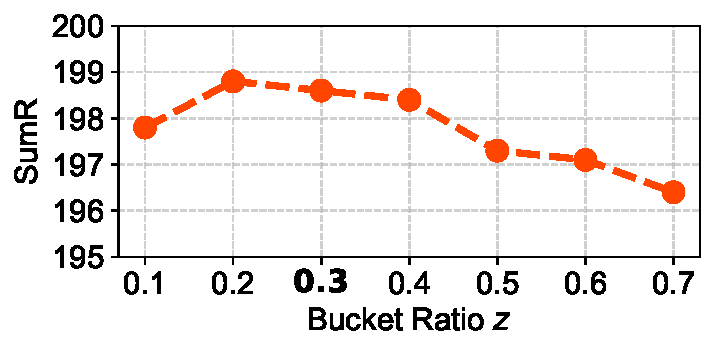
\includegraphics[width=\linewidth]{images/tvr_ratio-.pdf}
    }
    \hspace{0.02\textwidth}
    \vspace{-0.6em}
    \caption{The parameter analysis of the temperature $\tau$ in \cref{ea:evi1}, the threshold $\beta$ in \cref{eq:threshold}, and the dustbin bucket ratio $z$ in \cref{eq:new-s} on the TVR dataset, with the default settings highlighted in bold.
    }
    \label{fig:parameter_analysis}
\end{figure*}